	\chapter{Clustering} 	\resetquestioncounter{}
	\begin{qanda}
		\begin{question}
What are some applications of clustering in real-world scenarios?
		\end{question}

		\begin{answer}
Common applications of clustering include
	\begin{bulletedlist}
		\item Customer Segmentation
		\item Document Clustering
		\item Image Segmentation
		\item Recommendation Engines\end{bulletedlist}\end{answer}\end{qanda}



	\section{Clustering}
	\begin{bulletedlist}
		\item Clustering is an Unsupervised Learning Technique.
		\item A Cluster: collection of objects that are similar.
		\item Objective is to group similar data points into a group.
		\begin{bulletedlist}
			\item Segmenting customers into similar groups.
			\item Automatically organizing similar files/emails into folders.
		\end{bulletedlist}
		\item Simplifies data by reducing many data points into a few clusters.
		\item Some specific applications.
		\begin{bulletedlist}
			\item Image processing : used to cluster of pixels representing objects in each frame. The attributes of each pixel can include brightness, color, and location, the x and y
coordinates in the frame. Successive frames are examined to identify any changes to the clusters. These newly identified clusters may indicate unauthorized access to a facility.
			\item Medical : Patient attributes such as age, height, weight, systolic and diastolic blood pressures, cholesterol level, and other attributes can identify naturally occurring clusters under various health conditions.
			\item Customer segmentation : Cluster customers on basis of frequency of purchase, recency of purchase, value of purchase and look for common attributes among high value customers. Target all potential customers who have similar attributes.
		\end{bulletedlist}
	\end{bulletedlist}

	\subsection{Distance}
Do define ``similarity'' you need a measure of distance.  Examples of common distance measures.
	\begin{bulletedlist}
		\item Manhattan Distance
		\item Eucledian Distance
		\item Chebyshev Distance (also called the chess board distance)
		\item Minkowski with:
		\begin{bulletedlist}
			\item P=1 is Manhattan
			\item P=2 is Euclidean
			\item P=$\infty$ is Chebyshev
		\end{bulletedlist}
	\end{bulletedlist}

	\begin{bulletedlist}
		\item Choice of distance measures play a key role in cluster analysis.
		\item Knowledge of the distribution of data (gaussian or otherwise) will help.
		\item Are the various attributes independent or influence each other.
		\item Are their outliers in the data on the various dimensions.
		\item Though Euclidian distance is the most commonly used distance metric, it has three main features that should be kept in view.
		\begin{bulletedlist}
			\item It is highly scale dependent. Changing the units of one variable can have a huge influence on the results. Hence standardizing the dimensions is a good practice.
			\item It completely ignores the relationship between measurements.
			\item It is sensitive to outliers. If the data has outliers that cannot be handled or removed, use of Manhattan distance is preferred.
		\end{bulletedlist}
	\end{bulletedlist}


Mahalanobis distance attempts to capture the relationship between variables.  It finds the ``principal components,'' the eigenvectors of the data.  It forms ellipses along the eigenvector axes and uses those to define the distance.
	\begin{equation}
		\left(\mbf{x}-\bar{x}\right)^T \mbf{C}^{-1}\left(\mbf{x}-\bar{x}\right)
	\end{equation}
	\begin{mathwhere}
		\mathdefitem{\mbf{x}}{vector of points;}
		\mathdefitem{\bar{x}}{center of points;}
		\mathdefitem{\mbf{C}}{covariance matrix;}
	\end{mathwhere}

Jaccard distance defines a distance for groups of points.  It is
	\begin{equation}
		1 - J(A,B)
	\end{equation}
where
	\begin{equation}
		J(A,B) = \frac{\left|A\cap B\right|}{\left|A\cup B\right|}
	\end{equation}
The number of points in the intersection of A and B divided by the number of points in A union B.

	\subsection{Importance of Scaling}

	\begin{bulletedlist}
		\item Most distance measures are highly influenced by the scale of each variable.
		\item Variables with large scales have a much greater influence over the distance.
		\item Hence all measurements are converted to the same scale.  For example z-scores.
	\end{bulletedlist}

	\subsection{Types of Clustering}
Connectivity based clustering is expensive, but allows flexible segregation of clustering after the fact.
	\begin{displaymath}
		\frac{n(n+1)}{2}
	\end{displaymath}
Centroid base clustering is less expensive.
	\begin{displaymath}
		kn
	\end{displaymath}
	\begin{mathwhere}[0.38in]
		\mathdefitem{n}{number of samples;}
		\mathdefitem{k}{number of clusters.}
	\end{mathwhere}

	\subsubsection{Connectivity Based Clustering}
Connectivity based clustering (Hierarchical clustering): based on the idea that related objects are closer to each other. Can we then create a hierarchy of clusters/groups.
	\begin{bulletedlist}
		\item Hierarchical Clustering techniques create clusters in a hierarchical tree like structure.
		\item Any type of distance measure can be used as a measure of similarity.
		\item Cluster tree like output is called dendrogram.
		\item Techniques either start with individual objects and sequentially combine them (agglomerative), or start from one cluster of all objects and sequentially divide them (divisive).
		\item Useful when you want flexibility in how many clusters you ultimately want. For example, imagine grouping items on an online marketplace like Etsy or Amazon.
		\item In terms of outputs from the algorithm, in addition to cluster assignments you also build a nice tree (dendrogram) that tells you about the hierarchies between the clusters. You can then pick the number of clusters you want from this tree.
		\item In a dendrogram, the y-axis marks the distance at which the clusters merge, while the objects are placed along the x-axis.
		\item Algorithms can be agglomerative (start with 1 object and aggregate them into clusters) or divisive (start with complete data and divide into partitions).
	\end{bulletedlist}

	\begin{figure}[h]
		\centering
		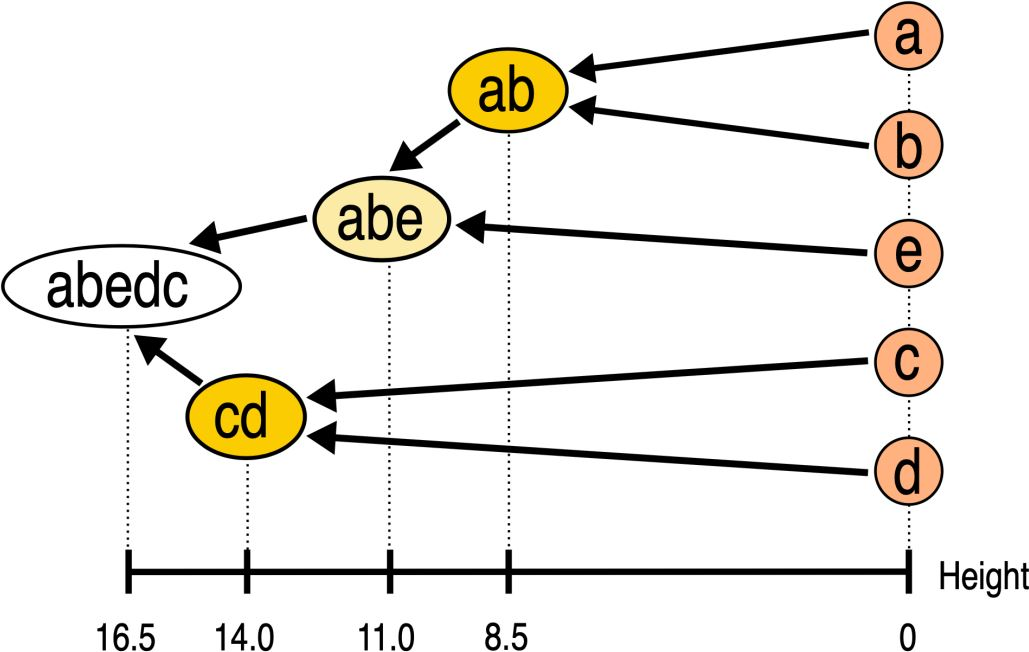
\includegraphics[height=2.5in]{clusteringdendrogram}
		\caption{Connectivity base clustering dendrogram.}
		\label{fig:clusteringdendrogram}
	\end{figure}

Starts with each object as a cluster of one record each.  Sequentially merges 2 closest records by distance as a measure of similarity to form a cluster.  Various measure can be used to determine distance between two clusters.
	\begin{figure}[h]
		\centering
		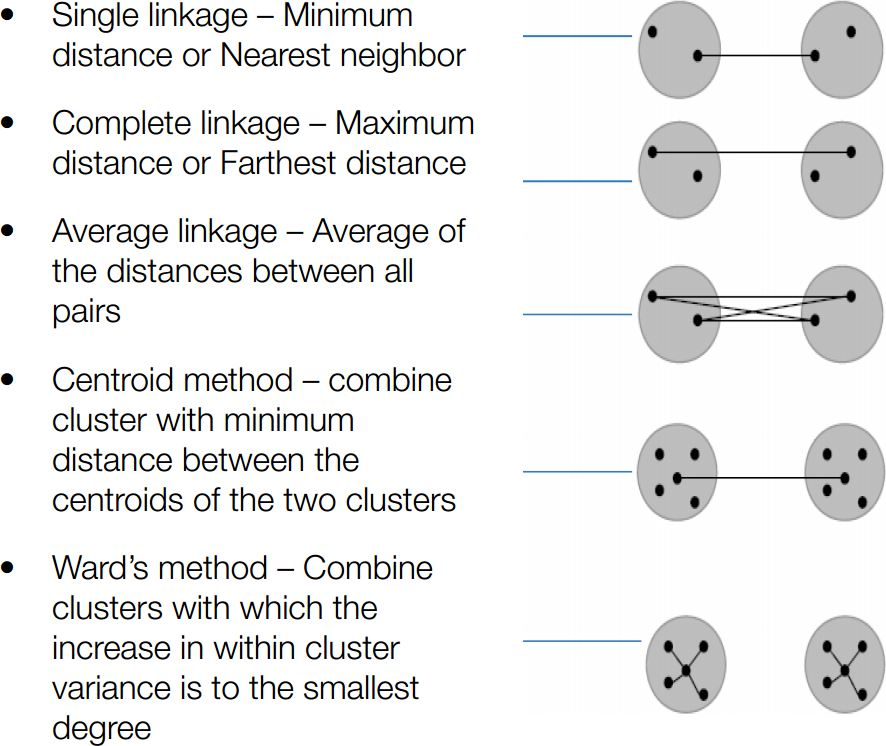
\includegraphics[height=3.5in]{distancemeasuresbetweenclusters}
		\caption{Distance measures between clusters.}
		\label{fig:distancemeasuresbetweenclusters}
	\end{figure}

	\subsubsection{Centroid Based Clustering}
Centroid based clustering (Eg. K-Means clustering): The objective is to find K clusters/groups. The way these groups are defined is by creating a centroid for each group. The centroids
are like the heart of the cluster, they ``capture'' the points closest to them and add them to the cluster.

	\begin{bulletedlist}
		\item Large K produces smaller groups and a small K produces larger groups.
		\item K-Means uses Euclidean distances and is the most popular.
		\item Other variants like K-medians and K-mediods use other distance measures.
	\end{bulletedlist}

	\subsection{K-Means Clustering}

	\begin{bulletedlist}
		\item K-Means is probably the most used clustering technique.
		\item Aims to partition the n observations into k clusters so as to minimize the within-cluster sum of squares (i.e. variance).
		\item Computationally less expensive compared to hierarchical techniques.
		\item Have to pre-define K, the no of clusters.
		\item Requires data to be scaled first.  The most popular method of scaling is to use z-scores.
	\end{bulletedlist}
